\documentclass[11pt]{article}
\usepackage[margin=1in]{geometry}
\usepackage{amsmath,amssymb,amsthm}
\usepackage{graphicx}
\usepackage{booktabs}
\usepackage{hyperref}

\newtheorem{proposition}{Proposition}
\newtheorem{lemma}[proposition]{Lemma}
\theoremstyle{remark}
\newtheorem{remark}[proposition]{Remark}

\title{A numerical look at the sextic family\\in the quasi-Riemann argument}
\author{Tommi Niilola}
\date{Draft, October 2026}

\begin{document}
\maketitle

\begin{abstract}
A recent preprint~\cite{OAI} proves that every Dirichlet $L$-function is zero-free in
$\operatorname{Re}s>11/12$. The key input is a mean-square estimate for a family of sextic
twists $A_u(D)$ of a Möbius sum over the Eisenstein integers, proved for row ranges
$N(u)\le H=D^{1+\vartheta}$. We record a short, self-contained form of the sixth-power
amplification of the companion $7/8$ paper~\cite[Lemma~17.6]{OAI78} as a conditional statement:
if the mean-square estimate holds for row ranges $H=D^\kappa$ with some $\kappa>0$, then
$L_K(s,\nu)$ is zero-free in $\operatorname{Re}s>\tfrac12+\tfrac{5\kappa}{12}$. Thus the row range is the single parameter that interpolates between the proved
exponent $11/12$ ($\kappa\to1$) and the Riemann Hypothesis ($\kappa\to0$). We also note why no
estimate for general coefficients can reach below $H=D$. We then compute the family directly for
$2{,}500\le D\le320{,}000$ (up to $9\times10^5$ rows). The normalised mean square equals $1$
to within the fluctuations of a random-sign control at every row range tested, including
$H=D^{1/2}$ to $D^{6/7}$, well below the range the proof reaches. Replacing $\mu$ by $1$
makes the family loud, as the preprint states. Finally, the Möbius rows have a tail
heavier than Gaussian: their fourth-moment ratio is $2.11$--$2.20$, against $2.00$ for
random signs. We show that this is predicted by the multiplicative energy of the columns, to
within $0.02$ for $D\ge5{,}000$. Repeating the test for cubic and quadratic twists, whose
mean-square inputs would give $5/6$ and $3/4$, shows the same quiet behaviour. The heavier tail is
the familiar non-Gaussian behaviour of random multiplicative functions, not a new effect.
Each row is the Möbius sum of a Hecke $L$-function. Using zeros computed with PARI/GP, the
explicit formula reproduces individual rows to within $1\%$, and over $726$ rows the mean square
matches the family average of $\sum_\rho|\widehat W(\rho)|^2/|L'(\rho)|^2$. The large values of this
sum come from close pairs of zeros. These pairs occur at the rate of random unitary matrices,
except on the thin set of rows whose $L$-functions factor. The computations use one smooth weight
and the trivial twist. Apart from the conditional proposition, all results are numerical and
exploratory, and they are consistent with the mean-square estimate without establishing it.
\end{abstract}

\section{The family and where its exponent comes from}

Let $K=\mathbb Q(\sqrt{-3})$ and $\mathcal O=\mathbb Z[\omega]$. For a smooth $W$ supported
in $[1,2]$, the preprint~\cite{OAI} considers
\[
A_u(D)=\sum_{\mathfrak n}\mu(\mathfrak n)\,\chi_{\mathfrak n}(u)\,W\!\big(N\mathfrak n/D\big),
\qquad \chi_{\mathfrak n}(u)=(u/\mathfrak n)_6,
\]
over ideals $\mathfrak n$ prime to $6$ (we take the twisting Hecke character $\nu$ trivial).
Its Proposition~3.1 states the mean-square bound
\begin{equation}\label{eq:ms}
\sum_{0<N(u)\le H}|A_u(D)|^2\ll D^{1+\varepsilon}H,\qquad H=D^{1+\vartheta},\ 0<\vartheta\le1/10.
\end{equation}
Because $\chi_{\mathfrak n}(p^6)=\mathbf 1_{\mathfrak p\nmid\mathfrak n}$, each row $u=p^6$
with $N(p)\approx Y=H^{1/6}$ is a copy of the target sum, $A_{p^6}=A_1+O(D/Y)$. Comparing the
$\asymp Y/\log Y$ copies with~\eqref{eq:ms} gives~\cite[Sec.~3]{OAI}
\begin{equation}\label{eq:extract}
|A_1(D)|^2\ll D^{1+\varepsilon}H^{5/6}+D^2H^{-1/3},
\end{equation}
hence $A_1(D)\ll D^{11/12+\varepsilon}$ for $H\approx D$. A Mellin argument converts this
into the zero-free half-plane.

Taken at face value with $H=D^\kappa$, \eqref{eq:extract} would stop at $\kappa=6/7$,
because the trivial bound $O(D/Y)$ for the copy error eventually dominates. That floor is
an artefact. The copy error is itself a Möbius sum of the same kind at a smaller scale, and
an induction over scales removes it. The $7/8$ paper~\cite[Lemma~17.6]{OAI78} removes it in the
same way, through a supremum over smaller scales, and for every row $u$ rather than only $u=1$.
Proposition~\ref{prop:cond} below is the special case $u=1$ written for a general row range.

\paragraph{Notation for this section.} Let $\nu$ be a finite-order Hecke character of $K$
and $S$ a finite set of prime ideals containing those above $2$, $3$ and the conductor of
$\nu$. For $W\in C_c^\infty((0,\infty);\mathbb C)$ and $X>0$ put
\[
A_u(X)=A_u(X;W)=\sum_{(\mathfrak n,S)=1}\mu(\mathfrak n)\nu(\mathfrak n)\chi_{\mathfrak n}(u)
W(N\mathfrak n/X),
\]
so $A_1(X)$ is the untwisted sum. We say that \emph{$\mathrm{MS}(\kappa)$ holds for $W$} if
for every $\varepsilon>0$
\begin{equation}\label{eq:msk}
\sum_{0<N(u)\le D^\kappa}|A_u(D;W)|^2\ll_{W,\varepsilon}D^{1+\kappa+\varepsilon}
\qquad(D\ge2).
\end{equation}
Proposition~3.1 of~\cite{OAI} is $\mathrm{MS}(1+\vartheta)$ for every
$0<\vartheta\le1/10$, and~\cite[(17.87)]{OAI78} gives $\mathrm{MS}(\kappa)$ for every $\kappa>1$,
uniformly over the twists, both signs of the symbol, and the rowwise profiles needed there.

\begin{proposition}\label{prop:cond}
Let $\kappa>0$, and suppose $\mathrm{MS}(\kappa)$ holds for $W$. Then for every
$\varepsilon>0$,
\[
A_1(D;W)\ll_{W,\varepsilon}D^{\frac12+\frac{5\kappa}{12}+\varepsilon}.
\]
Consequently, if $\mathrm{MS}(\kappa)$ holds for every $W\in C_c^\infty((1,2);\mathbb C)$,
then $L_K(s,\nu)$ has no zeros in $\operatorname{Re}s>\frac12+\frac{5\kappa}{12}$.
\end{proposition}

\begin{proof}
We may assume $\kappa<6/5$; otherwise the exponent is at least $1$ and the trivial bound
$\mathrm B(1)$ below suffices. Then $1-\kappa/6\in(4/5,1)$.
Fix $W$ with support in $[a,b]\subset(0,\infty)$. For $\theta\in[\frac12,1]$ let
$\mathrm B(\theta)$ be the statement that $|A_1(X;W)|\le C_\theta X^\theta$ for all $X>0$,
with $C_\theta$ depending only on $W$ and $\theta$. Since $A_1(X)=0$ for $X<1/b$ and
$|A_1(X)|\le\|W\|_\infty\#\{\mathfrak n:N\mathfrak n\le bX\}\ll_W\max(X,1)$, the statement
$\mathrm B(1)$ holds.

\emph{Step 1: the copy error as a Möbius sum.} Let $\mathfrak p\notin S$ be a prime ideal,
and for a function $f$ write $\Sigma[f]=\sum_{(\mathfrak m,S)=1}\mu\nu(\mathfrak m)f(N\mathfrak m)$
and $\Sigma_{\mathfrak p}[f]$ for the same sum restricted to $\mathfrak p\nmid\mathfrak m$.
Splitting according to whether $\mathfrak p\mid\mathfrak m$, and writing
$\mathfrak m=\mathfrak p\mathfrak m'$ in the second part, gives
$\Sigma[f]=\Sigma_{\mathfrak p}[f]-\nu(\mathfrak p)\Sigma_{\mathfrak p}[f(N\mathfrak p\,\cdot)]$.
Iterating (the sums vanish once the support of $f(N\mathfrak p^j\,\cdot)$ lies below $1$),
\[
\Sigma_{\mathfrak p}[f]=\sum_{j\ge0}\nu(\mathfrak p)^j\,\Sigma[f(N\mathfrak p^j\,\cdot)].
\]
Now let $p$ be a generator of $\mathfrak p$. Since $\chi_{\mathfrak n}(p^6)=1$ if
$\mathfrak p\nmid\mathfrak n$ and $0$ otherwise, and since $\mathfrak n=\mathfrak p\mathfrak m$
with $\mathfrak p\nmid\mathfrak m$ gives $\mu\nu(\mathfrak n)=-\nu(\mathfrak p)\mu\nu(\mathfrak m)$,
\[
E_{\mathfrak p}:=A_1(D)-A_{p^6}(D)
=-\nu(\mathfrak p)\,\Sigma_{\mathfrak p}\big[W(N\mathfrak p\,\cdot/D)\big]
=-\nu(\mathfrak p)\sum_{j\ge0}\nu(\mathfrak p)^j A_1\big(D/N\mathfrak p^{j+1}\big).
\]
This identity is exact.

\emph{Step 2: one round of extraction.} Assume $\mathrm B(\theta)$. Every prime ideal prime
to $6$ has norm at least $7$, and $\theta\ge\frac12$, so Step~1 gives
\[
|E_{\mathfrak p}|\le C_\theta\Big(\frac D{N\mathfrak p}\Big)^{\theta}
\sum_{j\ge0}7^{-j/2}\le2C_\theta\Big(\frac D{N\mathfrak p}\Big)^{\theta}.
\]
Let $H=D^\kappa$, $Y=H^{1/6}$, and let $\mathcal P$ be the set of prime ideals
$\mathfrak p\notin S$ with $Y/2<N\mathfrak p\le Y$, with generators $p$. The rows $p^6$ are
distinct and satisfy $N(p^6)\le H$. By Landau's prime ideal theorem
$J=\#\mathcal P\gg Y/\log Y$ for large $D$. For each $\mathfrak p\in\mathcal P$,
$|A_1|^2\le2|A_{p^6}|^2+2|E_{\mathfrak p}|^2$. Averaging over $\mathcal P$ and
using~\eqref{eq:msk},
\[
|A_1(D)|^2\le\frac2J\sum_{0<N(u)\le H}|A_u(D)|^2+32\,C_\theta^2\,D^{2\theta}Y^{-2\theta}
\ll_{W,\varepsilon}D^{1+\frac{5\kappa}6+2\varepsilon}+D^{2\theta(1-\frac\kappa6)}.
\]
Hence $\mathrm B(\theta)$ implies $\mathrm B(\theta')$ with
$\theta'=\max\big(\tfrac12+\tfrac{5\kappa}{12}+\varepsilon,\ \theta(1-\tfrac\kappa6)\big)$.

\emph{Step 3: iteration.} Start from $\theta_0=1$ and set
$\theta_{k+1}=\max(\frac12+\frac{5\kappa}{12}+\varepsilon,\ \theta_k(1-\frac\kappa6))$. Since
$1-\kappa/6<1$, after finitely many steps $\theta_k=\frac12+\frac{5\kappa}{12}+\varepsilon$.
Each step changes the constant by a factor depending only on $W$, $\kappa$ and $\varepsilon$,
so this proves the bound.

For the zero-free region, suppose $L_K(\varrho,\nu)=0$ with
$\operatorname{Re}\varrho>\frac12+\frac{5\kappa}{12}$. Take $W(y)=y^{-\varrho}\phi(y)$ with
$0\le\phi\in C_c^\infty((1,2))$ nonzero, and put $\widehat W(s)=\int_0^\infty W(y)y^{s-1}\,dy$.
For $\operatorname{Re}s>1$, substituting $X=N\mathfrak n/y$ termwise gives
\[
\int_0^\infty A_1(X;W)\,X^{-s}\,\frac{dX}{X}=\frac{\widehat W(s)}{L_K^S(s,\nu)},\qquad
L_K^S(s,\nu)=\prod_{\mathfrak p\notin S}\big(1-\nu(\mathfrak p)N\mathfrak p^{-s}\big)^{-1}.
\]
Since $A_1(X;W)=0$ for $X<1/2$ and $A_1(X;W)\ll X^{\theta}$ with
$\theta=\frac12+\frac{5\kappa}{12}+\varepsilon$, the left side is holomorphic in
$\operatorname{Re}s>\theta$, so the identity continues there. Now
$\widehat W(\varrho)=\int_1^2\phi(y)y^{-1}\,dy>0$, and
$L_K^S(s,\nu)=L_K(s,\nu)\prod_{\mathfrak p\in S}(1-\nu(\mathfrak p)N\mathfrak p^{-s})$, where the
finite product has no zeros in $\operatorname{Re}s>0$. So the right side has a pole at
$\varrho$ if $\operatorname{Re}\varrho>\theta$, a contradiction. Letting $\varepsilon\to0$ gives
the half-plane. This is the argument of~\cite[Sec.~3]{OAI}.
\end{proof}

\begin{remark}
(i) For $\kappa=1+\vartheta$ the proposition gives $\frac{11}{12}+\frac{5\vartheta}{12}$,
the exponent of~\cite{OAI}; the induction does not help there, because the copy error is
not the bottleneck. (ii) The exponent equals $6/7$ at $\kappa=6/7$, $5/6$ at
$\kappa=4/5$, and tends to $1/2$ as $\kappa\to0$. For each fixed $\kappa>0$ the row range
$D^\kappa$ still grows with $D$. The point is the limit: if $\mathrm{MS}(\kappa)$ held for
arbitrarily small $\kappa>0$, the zero-free regions would approach $\operatorname{Re}s=\frac12$,
which is the Riemann Hypothesis for $L_K(s,\nu)$. (iii) The
factor $\frac5{12}=\frac12(1-\frac16)$ comes from the density $H^{1/6}$ of the sixth-power
copies. A family built from characters of order $k$ would give
$\frac12+\frac\kappa2(1-\frac1k)$. (iv) The hypothesis cannot be weakened to the copy rows
alone. By Step~1 and the induction, the bound
$\sum_{\mathfrak p\in\mathcal P}|A_{p^6}(D)|^2\ll D^{1+\kappa+\varepsilon}$ over the copy rows of
Step~2 holds at every scale if and only if $A_1(D)\ll D^{\frac12+\frac{5\kappa}{12}+\varepsilon}$
at every scale. For all $W$, that bound is in turn equivalent to the zero-free half-plane:
one direction is the Mellin argument above, the other a contour shift to a line
$\operatorname{Re}s=\sigma_1+\eta$ strictly inside the zero-free half-plane
$\operatorname{Re}s>\sigma_1$. There $1/L_K(s,\nu)$ grows at most polynomially in $|\operatorname{Im}s|$, by the
Borel--Carath\'eodory argument of~\cite[\S14.2]{Titchmarsh}. Because $W$ is smooth and compactly
supported in $(1,2)$, its Mellin transform decays faster than every power of $|\operatorname{Im}s|$,
so a polynomial bound is enough for the shift. So the copy rows carry no
information beyond the conclusion. All the content of $\mathrm{MS}(\kappa)$ lies in the
non-copy rows, which supply the averaging that the copies then extract.
\end{remark}

The next lemma shows why the structure of $\mu$ is essential for row ranges below $D$.

\begin{lemma}\label{lem:general}
Let $\mathcal N$ be the set of squarefree ideals prime to $S$ with $D\le N\mathfrak n\le2D$.
There is no inequality
$\sum_{0<N(u)\le H}\big|\sum_{\mathfrak n\in\mathcal N}a_{\mathfrak n}\chi_{\mathfrak n}(u)\big|^2
\le C\,D^{\varepsilon}H\sum|a_{\mathfrak n}|^2$ valid for all coefficients when
$H\le D^{1-2\varepsilon}$ and $D$ is large.
\end{lemma}

\begin{proof}
Take $a_{\mathfrak n}=1$. The row $u=1$ alone contributes
$(\#\mathcal N)^2\gg D\cdot\#\mathcal N$, which exceeds $C D^{\varepsilon}H\,\#\mathcal N$
once $H\le D^{1-2\varepsilon}$ and $D$ is large.
\end{proof}

So for $H<D$, any proof of~\eqref{eq:msk} must use the arithmetic of $\mu$, as the identity
absorbing $\mu$ into cubic Gauss sums does in~\cite{OAI}. Heuristically, $H\approx D$ is
also where that argument stops. Poisson summation in $u$ turns rows of length $H$ into dual
rows of length $\asymp D^2/H$. Square-root cancellation on the dual side then contributes
$\approx D^2$, which is below the target $DH$ only when $H\ge D$. This is the familiar
$D+H$ barrier of large-sieve inequalities. In~\cite{OAI} it appears as the requirement, in
the cube-removal step, that the dual range be shorter than $D$ by a power. Going below it
requires cancellation beyond square-root among the dual coefficients, which are cubic Gauss
sums.

\paragraph{The barrier, measured.} For general coefficients the best possible constant in a
mean-square bound is $\Delta=\|M\|^2$, where $M_{u,\mathfrak n}=\chi_{\mathfrak n}(u)$, and
always $\Delta\ge\max(\#\text{rows},\#\text{cols})$. We computed $\Delta$ exactly, as the top
eigenvalue of $M^{*}M$, for $D=2{,}500$, $5{,}000$, $10{,}000$ and row ranges
$H=D^{0.5},\dots,D^{1.0}$. In every case $\Delta$ is between $1.58$ and $2.37$ times
$\#\text{rows}+\#\text{cols}$, while the Möbius vector $\mu W$ attains only $0.87$ to $1.03$
times $\#\text{rows}$. Removing the rows that duplicate other rows (those divisible by
$\lambda^6$ or $2^6$) does not change $\Delta$ noticeably. So a bound that treats $\mu$ as an
arbitrary vector overshoots the truth by a factor of about $(H+D)/H$. At $\kappa=1$ this is a
constant, about $2$; at $\kappa=1/2$ it is $8.0$, $12.9$ and $15.6$ for the three values of
$D$, growing like $D^{1-\kappa}$. This is the $D+H$ barrier in concrete form: below $H=D$ the
whole gain has to come from the arithmetic of $\mu$.

The singular vectors show what that gain consists of. For $H<D$ the matrix $M^*M$ has rank
equal to the number of rows, and its nonzero eigenvalues are all of size about $D$: at
$D=2{,}500$ and $5{,}000$ their mean is $0.94$ to $0.95$ times the number of columns, and the top
ten agree to within $20\%$. The top singular vectors are not attached to individual rows; at
most $2\%$ of the top left singular vector lies on any single row. So there are no special
directions for $\mu$ to avoid. Instead
$\sum_u|A_u|^2=\|Mc\|^2\approx D\,\|Pc\|^2$, where $c=\mu W$ and $P$ is the orthogonal
projection onto the span of the conjugated rows $\mathfrak n\mapsto\overline{\chi_{\mathfrak n}(u)}$,
$N(u)\le H$. For $H<D$, $\mathrm{MS}(\kappa)$ therefore says that $c$ puts no more than its
proportional share, about $H/D$ up to $D^\varepsilon$, of its mass into this $H$-dimensional space
of characters. Numerically, that is what happens. At $D=5{,}000$ the share is $0.171$ and $0.413$
for $\kappa=0.5$ and $0.6$, against $0.178$ and $0.420$ for the proportional value (rank divided
by the number of columns). Random-sign vectors give the same to within $\pm0.01$, and at
$D=2{,}500$ the agreement is equally close. A general vector can instead lie entirely in that
space, which is the factor $D/H$ lost by bounds for general coefficients.

This raises a concrete numerical question: \emph{does~\eqref{eq:ms} behave as a true
statement for row ranges $H<D$?}

\section{Computation}

We compute in $\mathcal O$ directly. Prime ideals prime to $6$ are the kernels of the maps
$\mathcal O\to\mathbb F_p$, $\omega\mapsto r$, for $p\equiv1\pmod 3$ and $r$ a primitive cube
root of unity (two ideals per $p$), and the inert ideals $(q)$, $q\equiv2\pmod3$, with
residue field $\mathbb F_q[\omega]$. For $\mathfrak p\nmid u$, $(u/\mathfrak p)_6$ is the
sixth root of unity congruent to $u^{(N\mathfrak p-1)/6}$, identified through
$\zeta_6=1+\omega$. The columns are all squarefree $\mathfrak n$ with
$D\le N\mathfrak n\le2D$, and the rows are all nonzero $u\in\mathcal O$ with $N(u)\le D^{1.1}$
(fewer for the two largest $D$). We use $W(x)=\exp(1-1/(1-(2x-3)^2))$ on $(1,2)$.

\paragraph{Checks.} Before measuring, we verify: multiplicativity in $u$; that the symbol
sums to zero over $\mathcal O/\mathfrak p$ and takes all six values; that its quadratic and
cubic parts reproduce the Legendre symbol and cubic residuosity of rational integers;
\emph{cubic reciprocity} $(\pi_1/\pi_2)_3=(\pi_2/\pi_1)_3$ for $1{,}742$ pairs of primary
primes, which tests the identification of the sixth roots of unity; and the count of
squarefree ideals of norm $\le3000$ against an independent count of elements. All pass.

\paragraph{Normalisation.} For each row we record $\mathrm{mass}_u=\sum_{(\mathfrak n,u)=1}
|\mu(\mathfrak n)W(N\mathfrak n/D)|^2$, the value of $\mathbb E|A_u|^2$ in the random model,
and report
\[
R(\kappa)=\frac{\sum_{N(u)\le D^\kappa}|A_u|^2}{\sum_{N(u)\le D^\kappa}\mathrm{mass}_u},
\]
so that $R=1$ is exact square-root cancellation. As controls, we repeat the computation
with $\mu(\mathfrak n)$ replaced by independent random signs (same columns and rows) and by
$1$.

\section{Results}

\paragraph{Mean square.} Table~\ref{tab:R} and Figure~\ref{fig:family}(a) show $R(\kappa)$.
For every $D$ and every row range from $H=D^{1/2}$ to $D^{1.1}$, $R$ lies within $0.92$ to
$1.09$. The spread is largest at small $\kappa$, where there are fewest rows, and it is the
same size as the spread of the random-sign control (grey band). At $\kappa=6/7$, where
Proposition~\ref{prop:cond} would give the exponent $6/7$, $R=0.999$ at $D=320{,}000$. We see
no sign of the mean square growing like a power of $D/H$ below $H=D$.

\begin{table}[t]
\centering
\small
\begin{tabular}{rrcccccc|c}
\toprule
$D$ & rows & $\kappa=0.5$ & $0.6$ & $0.7$ & $6/7$ & $1.0$ & $1.1$ & random, $6/7$ \\
\midrule
\csname @@input\endcsname tab_R.tex
\bottomrule
\end{tabular}
\caption{Normalised mean square $R(\kappa)$ of the Möbius family for row ranges $H=D^\kappa$.
The last column is the random-sign control at $\kappa=6/7$.}
\label{tab:R}
\end{table}

\paragraph{The Möbius function matters.} With $\mu$ replaced by $1$, $R(0.5)$ is $5.0$, $9.3$
and $17.9$ at $D=5{,}000$, $20{,}000$ and $80{,}000$, growing with $D$. The largest rows are
$u=1$, $u=2^6$ and $u=-27$, which are exact copies, and each carries $|A_u|^2\approx D/5$
times its mass. This illustrates the preprint's remark that the argument genuinely needs the
Möbius signs.

\paragraph{Tails and multiplicative energy.} The distribution of
$z=|A_u|^2/\mathrm{mass}_u$ is not exactly Gaussian for the Möbius family. At $D=80{,}000$,
$3.5\times10^{-4}$ of the rows with $N(u)\le D$ have $z>10$, against $4\times10^{-5}$ for
random signs (the complex-Gaussian value is $e^{-10}=4.5\times10^{-5}$). The fourth-moment
ratio $\mathbb E|A_u|^4/(\mathbb E|A_u|^2)^2$ is $2.11$--$2.20$, growing slowly with $D$,
against $2.00$--$2.02$ for random signs (Table~\ref{tab:m4}, Figure~\ref{fig:family}(b)).
Within each run, the excess is roughly the same in every range of $N(u)$ from $10^2$ to
$10^5$ (for example $2.15$--$2.18$ at $D=80{,}000$), so it does not depend noticeably on the
conductor of the row.

The explanation is arithmetic. If the rows average $\chi_{\mathfrak n}(u)$ like independent
random sixth roots of unity at each prime, then
$\mathbb E|A_u|^4=\sum_{\mathfrak m}\big(\sum_{\mathfrak n_1\mathfrak n_2=\mathfrak m}
c(\mathfrak n_1)c(\mathfrak n_2)\big)^2$ with $c=\mu W$. Besides the diagonal solutions,
which give the Gaussian value $2$, this counts the solutions of
$\mathfrak n_1\mathfrak n_2=\mathfrak n_3\mathfrak n_4$. For squarefree solutions
$\mu(\mathfrak n_1)\mu(\mathfrak n_2)\mu(\mathfrak n_3)\mu(\mathfrak n_4)=+1$, so they add
rather than cancel. With independent random signs they cancel. We computed this
multiplicative energy exactly for $D\le20{,}000$, hashing ideals by their prime factors. It
matches the measured ratio to within $0.02$ for $D\ge5{,}000$, and to $0.06$ at $D=2{,}500$,
where the finite row range is a coarser approximation to exact orthogonality
(Table~\ref{tab:m4}). This is the same mechanism
that makes the fourth moment of a random multiplicative function exceed its Gaussian
value~\cite{ACZ,Harper}. It does not affect the mean square.

\begin{table}[t]
\centering
\small
\begin{tabular}{rccc}
\toprule
$D$ & Möbius (measured) & energy prediction & random signs (measured) \\
\midrule
\csname @@input\endcsname tab_m4.tex
\bottomrule
\end{tabular}
\caption{Fourth-moment ratio $\mathbb E|A_u|^4/(\mathbb E|A_u|^2)^2$ over all rows.}
\label{tab:m4}
\end{table}

\begin{figure}[t]
\centering
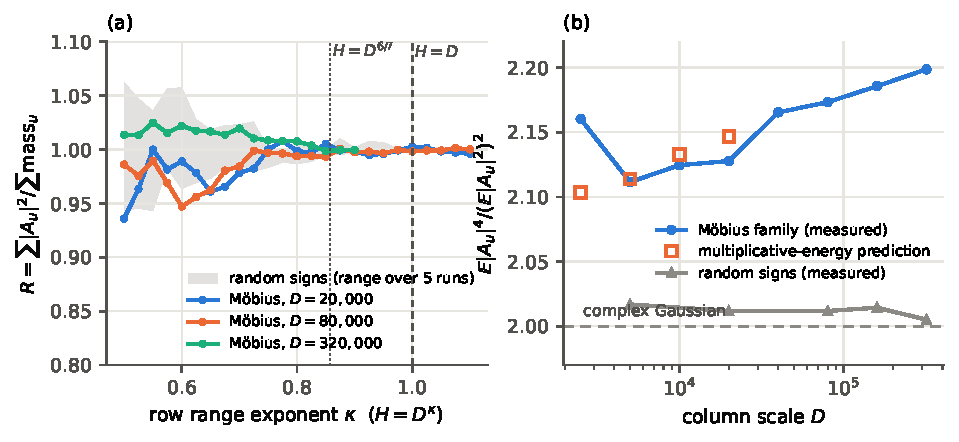
\includegraphics[width=\textwidth]{fig_family.pdf}
\caption{(a) Normalised mean square against the row-range exponent, for three column scales,
with the range of five random-sign controls in grey. (b) Fourth-moment ratio of the rows:
Möbius family, multiplicative-energy prediction, and random-sign control.}
\label{fig:family}
\end{figure}

\section{Families of lower order}\label{sec:order}

For $k\in\{2,3,6\}$ put
\[
A^{(k)}_u(D)=\sum_{(\mathfrak n,S)=1}\mu(\mathfrak n)\nu(\mathfrak n)\,
\chi_{\mathfrak n}(u)^{6/k}\,W(N\mathfrak n/D),
\]
so $k=6$ is the sextic family, $k=3$ uses the cubic symbol $(u/\mathfrak n)_3$ and $k=2$ the
quadratic symbol $(u/\mathfrak n)_2$. The copies are now the rows $u=p^k$, because
$\chi_{\mathfrak n}(p^k)^{6/k}=\chi_{\mathfrak n}(p)^6=\mathbf 1_{\mathfrak p\nmid\mathfrak n}$.
The proof of Proposition~\ref{prop:cond} goes through unchanged with $6$ replaced by $k$: the
copies have density $Y=H^{1/k}$, and the induction factor becomes $1-\kappa/k$. Hence:

\begin{proposition}\label{prop:order}
If the mean-square bound~\eqref{eq:msk} holds for $A^{(k)}_u$ with row range $D^\kappa$ for
every $W\in C_c^\infty((1,2);\mathbb C)$, then $L_K(s,\nu)$ has no zeros in
$\operatorname{Re}s>\frac12+\frac\kappa2\big(1-\frac1k\big)$.
\end{proposition}

At $\kappa=1$ this gives $11/12$, $5/6$ and $3/4$ for $k=6,3,2$. Table~\ref{tab:order}
repeats the experiment of Section~3 for the three families, with the plain control
($\mu$ replaced by $1$) for each. All three Möbius families are quiet at every row range
from $D^{1/2}$ to $D$. The plain families become louder as the copies become denser, and in
the same order as their densities $H^{1/6}$, $H^{1/3}$, $H^{1/2}$. The quadratic symbols are
real, so the Gaussian value of the fourth-moment ratio for $k=2$ is $3$ rather than $2$.
The excess above that value is also predicted. For real characters the fourth moment counts
solutions of $\mathfrak n_1\mathfrak n_2\mathfrak n_3\mathfrak n_4=\square$, and the exact
count at $D=20{,}000$ gives $3.445$, against a measured $3.452$. The excess, $0.445$, is
three times the complex excess $0.147$ at the same $D$, because all three pairings of the four
indices now contribute. Numerically, then, the mean-square inputs for $5/6$ and $3/4$ look as
true as the one proved in~\cite{OAI}.

The plain rows give a quantitative check of the copy count. If the $\asymp H^{1/k}$ copies
each carry $|A_u|^2\asymp D^2$, then $R_{\rm plain}-1\asymp D^{1-\kappa(1-1/k)}$, so at
$D=80{,}000$ the excess should shrink by $80{,}000^{0.1(1-1/k)}$ per step $0.1$ in $\kappa$.
For $k=2$ the successive ratios in Table~\ref{tab:order} are $1.69$ to $1.84$, against a
predicted $1.76$. For $k=3$ they are $1.69$ to $2.33$, against $2.12$. For $k=6$ this
asymptotic count does not apply at our sizes. The only copies with $N(u)\le D^{1.1}$ are
$u=1$, $\lambda^6=-27$ and $2^6=64$, because the next candidate has norm $7^6>10^5$. Removing
these two or three rows brings $R_{\rm plain}-1$ to between $-0.25$ and $-0.05$. So the
sextic plain excess at $\kappa=1$, $0.136$ at $D=20{,}000$ and $0.132$ at $D=80{,}000$, comes
from a fixed number of rows. The growth like $D^{1/6}$ only sets in once primes of norm at
least $7$ contribute copies.

\begin{table}[t]
\centering
\small
\setlength{\tabcolsep}{4pt}
\begin{tabular}{lrccccccc}
\toprule
family & $D$ & $\kappa=0.5$ & $0.6$ & $0.7$ & $0.8$ & $0.9$ & $1.0$ & 4th mom. \\
\midrule
\csname @@input\endcsname tab_order.tex
\bottomrule
\end{tabular}
\caption{Normalised mean square $R(\kappa)$ for the families of order $k=6,3,2$, with
Möbius coefficients and with $\mu$ replaced by $1$. The last column is
$\mathbb E|A_u|^4/(\mathbb E|A_u|^2)^2$ over rows with $N(u)\le D$.}
\label{tab:order}
\end{table}

\paragraph{Why the proof uses $k=6$ (partly heuristic).} The difference between the orders
appears after Poisson summation in $u$, which brings in Gauss sums of order $k$. Write
$\gamma_j$ for the normalised Gauss sums of~\cite{OAI}. Lemma~4.1 of~\cite{OAI} gives
$\gamma_2^3=\mu\alpha$ and $|\gamma_2|=1$ on squarefree $n$.
\begin{itemize}
\item $k=6$: the dual coefficients are $\mu\gamma_{-1}$, and by~\cite[(4.5)]{OAI}
  $\mu\gamma_{-1}=\chi_n(-1)G^{-1}\overline\alpha\gamma_2$. This is a cubic Gauss sum without
  $\mu$, hence a coefficient of Kubota's cubic theta function. Its transformation law turns
  the row twists into quadratic characters, so the quadratic large sieve applies and the
  extra $(ML)^{2/3}$ term of general higher-order large sieves is avoided, as~\cite{OAI}
  explains.
\item $k=3$: the dual coefficients are $\mu\gamma_{-2}=\mu\overline{\gamma_2}$. By the
  second identity in~\cite[(4.2)]{OAI}, $\mu\overline{\gamma_2}=\overline\alpha\,\overline G\,\gamma_1$:
  an \emph{unweighted sextic} Gauss sum times fixed phases. (The identity runs both ways:
  $\mu$ times a sextic sum is a cubic sum, and $\mu$ times a cubic sum is a sextic sum.) This
  leaves two routes, each with a known obstacle. Absorbing $\mu$ lands on sextic Gauss sums.
  These would be coefficients of a theta function on the six-fold metaplectic cover, and
  unlike the two- and three-fold covers, those coefficients are not known explicitly.
  Keeping cubic Gauss sums means keeping $\mu$. On primes, $\mu(\pi)\gamma_2(\pi)=-\gamma_2(\pi)$
  inherits Patterson's bias, and the resulting bilinear forms are the bottleneck
  of~\cite{HB00,DR}. Either way one ends up needing a large sieve for cubic twists, whose
  extra term Dunn and Radziwiłł showed is sharp up to $X^{o(1)}$~\cite{DR}. The obstruction
  is structural. It is \emph{not} a bias in the full sum of the dual coefficients, as the
  check below shows.
\item $k=2$: the Gauss sum of a quadratic character is $\sqrt{N\mathfrak n}$ times a simple
  factor, so the dual problem is again a Möbius sum twisted by quadratic characters, of the
  same length. The argument does not progress.
\end{itemize}

\paragraph{Checks.} (i) We evaluated $\gamma_1,\gamma_2,\gamma_3,\gamma_{-1}$ by complete
sums over residue systems, using no multiplicativity, for all $5{,}646$ squarefree primary
$n$ prime to $6$ with $N(n)\le20{,}000$. Every identity of~\cite[Lemma~4.1]{OAI} that
involves only these sums holds to within $10^{-12}$, including the evaluation of
$\gamma_3$ through the quadratic Gauss sum. Deliberately wrong variants fail (removing
$\mu$ breaks~(4.5) exactly when $\mu(n)=-1$). (ii) With the twisted multiplicativity
$\gamma_2(ab)=\gamma_2(a)\gamma_2(b)\chi_a(b)^2\chi_b(a)^2$, itself checked against complete
sums to $10^{-13}$, we computed $\gamma_2$ for all squarefree $n$ with $N(n)\le10^6$. The
prime sum $\sum_{N\mathfrak p\le X}\gamma_2(\mathfrak p)$ reproduces Patterson's
bias~\cite{HB00,DR}: it is real and positive, and $|S|/(X^{5/6}/\log X)$ stays between
$0.76$ and $0.86$ for $10^4\le X\le10^6$. The sum $\sum\gamma_2(n)$ over squarefree $n$ is
$(0.197\pm0.004)X^{5/6}$. In contrast, the Möbius-weighted sum
$\sum\mu(n)\overline{\gamma_2(n)}$, which gives the $k=3$ dual coefficients, stays between
$7$ and $184$ in absolute value and changes sign. That is at most the square root of the
number of terms ($2.8\times10^5$ at $X=10^6$), so it shows no bias.

\section{Rows as sums over zeros}\label{sec:rows}

\paragraph{The row $u=1$.} The zero-density reading of $\mathrm{MS}(\kappa)$ (Section~\ref{sec:disc}) treats
each row as a sum over the zeros of an $L$-function. For the row $u=1$ this can be tested
exactly. Grouping ideals by norm, $A_1(D)=\sum_m a(m)W(m/D)$ with
$\sum a(m)m^{-s}=1/\zeta_K^{(6)}(s)$, where $\zeta_K^{(6)}(s)=\zeta(s)L(s,\chi_{-3})
(1-4^{-s})(1-3^{-s})$. We computed $A_1(D)$ for $3{,}000$ values of $D$ between $10^2$ and
$10^7$ and compared it with the explicit formula
\[
A_1(D)=\sum_{\rho}\frac{\widehat W(\rho)D^{\rho}}{\zeta_K^{(6)\prime}(\rho)}
+\big(\text{poles of }1/\zeta_K^{(6)}\text{ on }\operatorname{Re}s=0\big),
\]
summed over the zeros of $\zeta$ and of $L(s,\chi_{-3})$ with $|\gamma|\le100$, without any
fitted parameter. The difference is $0.7\%$ to $1.2\%$ of the root-mean-square size of
$A_1(D)/\sqrt D$ on every range $D\ge10^2$, and the correlation is $0.99997$. Without the
terms on $\operatorname{Re}s=0$, which come from the removed Euler factors and are of size
$\log D$, the agreement holds only at large $D$ (residual $7\%$ for $D\ge10^6$).

\paragraph{Other rows.} The same test works for other rows. For fixed $u$, $\mathfrak n\mapsto(u/\mathfrak n)_6$ is a
Hecke character $\psi_u$ of $K$ (the Artin character of $K(u^{1/6})/K$), and
$A_u(D)=\sum_m a_u(m)W(m/D)$ with $\sum a_u(m)m^{-s}=1/L^{S}(s,\psi_u)$, $S$ the primes
dividing $6u$. We computed $a_u$ from the sextic symbols used in the family code (checked
against the family sums to $10^{-13}$). Separately, PARI/GP~2.19 identified the primitive
character from its values at primes up to $3000$, then computed the zeros of $L(s,\psi_u)$ with
$|\gamma|\le100$, the values $L'(\rho)$, and the poles on $\operatorname{Re}s=0$ coming from
$s=0$ and the removed Euler factors. For $u=2,-1,\omega,3+\omega,4+\omega,5$ (conductor norms
$576,16,27,3024,351,225$; $230$ to $403$ zeros each), the explicit formula reproduces
$A_u(D)/\sqrt D$ for $10^2\le D\le10^7$ with residual $0.17\%$ to $0.8\%$ and
$|$correlation$|\ge0.99997$ on every range, again without fitted parameters. Two rows needed
care, which is itself instructive. For $u=-1$ and $u=\omega$ the character factors through the
norm ($\psi_{-1}=\chi_{-4}\circ N$), so $L(s,\psi_u)=L(s,\chi)L(s,\chi\chi_{-3})$ is a product of
two Dirichlet $L$-functions. Their zeros do not repel each other, and nearly coincident pairs
occur ($\gamma=12.966$ and $12.988$ for $u=-1$; $9.565$ and $9.621$ for $u=\omega$). The
residues $\widehat W(\rho)/L'(\rho)$ at such pairs are large: the ``spectral mass''
$\sum_\rho|\widehat W(\rho)/L'(\rho)|^2$ is $0.63$ and $0.52$, against $0.10$--$0.11$ for the
four rows whose characters do not come from $\mathbb Q$ (random-model mass $0.12$--$0.14$).
If all nontrivial zeros of $L(s,\psi_u)$ lie on the critical line and are simple, Parseval
makes the spectral mass the long-run average of $|A_u(D)|^2/D$ over $\log D$. A zero with real
part $\beta\ne\frac12$ would instead contribute a term of size $D^{\beta-1/2}$ to
$A_u(D)/\sqrt D$, and a multiple zero adds powers of $\log D$. So this interpretation assumes
the Riemann Hypothesis for the row $L$-functions. Our computations use only the zeros on the
line up to the stated heights. The zero counts below are consistent with none missing there,
but they are not a certificate of completeness. So, row by row, $\mathrm{MS}(\kappa)$ is a statement about the family average
of a discrete negative moment $\sum_\rho|\widehat W(\rho)|^2/|L'(\rho)|^2$, and rows whose
$L$-functions factor are where that moment is large.

\paragraph{The family average.} We tested this over the family. For all $204$ rows with $1<N(u)\le60$, PARI computed the zeros
with $|\gamma|\le50$ (beyond that height the spectral mass changes by about $10^{-4}$ of its
value, checked on three rows at height $100$). The family mean of the spectral mass is
$0.1196$. The mean of $|A_u(D)|^2/D$ over the same rows is $0.1213$, $0.1184$ and $0.1166$ at
$D=10^4,10^5,10^6$, and $0.1193$ when each row is first averaged over $300$ values of
$D\in[10^3,10^6]$. The random-model mass is $0.130$, so $R\approx0.9$ on these small rows. Row
by row, the ratio of the $\log D$ average to the spectral mass has median $1.02$ and lies in
$[0.86,1.22]$ for $80\%$ of the rows. The outliers are rows with two zeros very close together.
For example, $u=8+2\omega$ has zeros at $\gamma=3.738$ and $3.786$; its character does not
come from $\mathbb Q$. The spectral mass there is $0.75$, but the beat period $2\pi/0.047$ in
$\log D$ is much longer than the window, so the window average is only $0.25$. Thus the mean
square of the family is reproduced, to about $2\%$, by the family average of
$\sum_\rho|\widehat W(\rho)|^2/|L'(\rho)|^2$. The distribution of this quantity over rows is
skewed (quantiles $0.090$, $0.107$, $0.148$ at $10\%$, $50\%$, $90\%$), and its upper tail
comes from small gaps between zeros. On this reading, $\mathrm{MS}(\kappa)$ asks that small
gaps, and the resulting small values of $|L'(\rho)|$, are not too frequent across the
family, while the zero-density reduction above concerns zeros off the line. Both are
statements about the zeros of the family, which is consistent with the reduction, but we
have no proof in either direction.

\paragraph{Where the tail comes from.} Extending to all $726$ rows with $1<N(u)\le200$ (conductor norms up to $8.6\cdot10^4$) shows
where the tail comes from. For every row, the number of zeros found differs from the main
term $\frac{2T}{\pi}\log\frac{T\sqrt q}{2\pi e}$ of the zero-counting formula ($T=50$, $q=3N(\mathfrak f)$ the
conductor over $\mathbb Q$ of a character with ideal conductor $\mathfrak f$; the conductor norms quoted above are $N(\mathfrak f)$) by between $-3.9$ and $+1.3$, with mean $0.03$. Differences of this size are what the
argument term $S(T)$ allows, so the counts are consistent with no missed zeros, and the close pairs are
unlikely to be artefacts. This is a consistency check, not a certified count. PARI/GP's
\texttt{lfunzeros} does not certify completeness, and we did not run a Turing-type verification.

Which rows factor can be decided exactly. Complex conjugation gives
$\psi_u(\bar{\mathfrak p})=\overline{\psi_{\bar u}(\mathfrak p)}$, so $\psi_u$ is invariant under
$\mathfrak p\mapsto\bar{\mathfrak p}$ (equivalently, factors through the norm, making
$L(s,\psi_u)$ a product of two Dirichlet $L$-functions) exactly when
$\psi_u\psi_{\bar u}=\psi_{N(u)}$ is trivial. By Kummer theory this happens exactly when $N(u)$
is a sixth power in $K$, that is, $N(u)=c^6$ with $c\in\mathbb Z$. Examples are the units, the
associates of $c^3$, and rows such as $\pi^4\cdot7$ with $N(\pi)=7$; we confirmed the criterion
numerically on these and on non-examples such as $\pi^3\cdot7$. Up to height $H$ there are
$H^{1/6+o(1)}$ such rows, a vanishing proportion. That alone does not make their contribution
to the mean square negligible, since a sparse set of rows can dominate if its members are
large enough; that would need a separate bound for these rows. Among
$1<N(u)\le200$ they are exactly the six associates of $8$. Write
$M_u=\sum_\rho|\widehat W(\rho)|^2/|L'(\rho)|^2$ and let
$\mathrm{diag}_u=\sum_m|a_u(m)|^2W(m/D)^2/D$ be the diagonal of the norm-grouped sum. Five
of the six factored rows have $M_u/\mathrm{diag}_u$ between $1.9$ and $5.2$, and the sixth
has $0.33$. For the other $720$ rows, the family mean of the spectral mass is $0.133$, the mean
of the $\log D$ averages is $0.125$, and the random-model mass is $0.130$ (median spectral mass
$0.110$). The $6\%$ gap between $0.133$ and $0.125$ is in the direction of the finite-window
effect just described. The spectral mass has a heavy upper tail. A Hill estimate of the tail
index of $M_u/\mathrm{diag}_u$ gives $1.3$ from the top $20$ rows and $2.1$ from the top $40$. In a GUE model, a gap of length $s$ between neighbouring zeros has
density $\propto s^2$ for small $s$ and makes $|L'(\rho)|\propto s$, so
$\Pr(|L'(\rho)|^{-2}>x)\propto x^{-3/2}$: finite mean, infinite variance. This is the
random-matrix explanation, due to Hughes, Keating and O'Connell~\cite{HKO}, of why the discrete
negative moments $\sum_{\gamma\le T}|\zeta'(\rho)|^{-2k}$ of Gonek and Hejhal~\cite{Gonek} are
expected to change behaviour at $k=3/2$. For the factored rows, where gaps are Poisson-like, the
corresponding exponent is $1/2$. The data are consistent with this, though $720$ rows cannot pin
the exponent down.

Two consequences follow. First, at fixed $D$ the mean square does not see the tail. If
$L(s)\approx(s-\rho_1)(s-\rho_2)g(s)$ near a close pair with gap $\Delta\gamma$, then
$L'(\rho_2)\approx-L'(\rho_1)$, and the two terms of the explicit formula nearly cancel:
\[
\frac{\widehat W(\rho_1)D^{\rho_1}}{L'(\rho_1)}+\frac{\widehat W(\rho_2)D^{\rho_2}}{L'(\rho_2)}
\approx\frac{\widehat W(\rho_1)D^{\rho_1}}{L'(\rho_1)}\big(1-D^{i\Delta\gamma}\big),
\]
whose squared size divided by $D$ is $|\widehat W(\rho_1)/L'(\rho_1)|^2\,4\sin^2(\frac12\Delta\gamma\log D)
\ll|\widehat W(\rho_1)/g(\rho_1)|^2(\log D)^2$. The spectral mass replaces $4\sin^2$ by its mean value
$2$ and so grows like $(\Delta\gamma)^{-2}$. At fixed $D$, the factor $\sin^2$ cuts off pairs with
$\Delta\gamma\lesssim1/\log D$; even a double zero would contribute only $O((\log D)^2)$. For
$u=8+2\omega$ the two residues have ratio $-0.93-0.24i$, and over $6.9\le\log D\le13.8$ the pair
contributes $0.11$ to $0.25$ to $|A_u(D)|^2/D$, against $0.66$ in $M_u$. Second, in this picture
$\mathrm{MS}(\kappa)$ is safe as long as the zeros of the family repel each other. Rows without
repulsion are the obvious threat, and in this family they are confined to the thin set
where $N(u)$ is a sixth power.

\paragraph{Repulsion, zero by zero.} The repulsion can be checked zero by zero rather than row by row. Take the $119{,}514$ zeros of
the $720$ generic rows with $3<|\gamma|<45$, unfold them with the density
$\frac1{2\pi}\log(q(\gamma/2\pi)^2)$, with $q=3N(\mathfrak f)$ as above. After unfolding, the
nearest-neighbour gap (the smaller of the two gaps next to a zero) has mean $0.737$, and we
then divide by this empirical mean. The fractions of normalised gaps below
$\varepsilon=0.05,0.1,0.2,0.4$ are $(1.3\pm0.4)\cdot10^{-4}$, $(9.4\pm1.3)\cdot10^{-4}$,
$(6.2\pm0.3)\cdot10^{-3}$ and $(3.95\pm0.09)\cdot10^{-2}$. The errors come from resampling whole
rows, since gaps within one $L$-function are correlated. For Haar unitary matrices of size $20$ and $60$ the corresponding fractions are
$1.3$ and $0.8\cdot10^{-4}$, $7.7$ and $9.8\cdot10^{-4}$, $6.0$ and $6.9\cdot10^{-3}$, and $4.9$
and $5.1\cdot10^{-2}$, with mean gap $0.725$. At the matched size $N=10$ they are $0.8\cdot10^{-4}$,
$8.4\cdot10^{-4}$, $6.0\cdot10^{-3}$ and $4.9\cdot10^{-2}$. Below $\varepsilon=0.2$ the family agrees
with CUE within the errors. At $\varepsilon=0.4$ it has about $20\%$ fewer gaps, matching its
slightly larger mean gap. The $784$ zeros of the factored rows give $3.6$,
$7.1$, $9.7$ and $21\cdot10^{-2}$ with mean gap $0.544$, against $2.8$, $5.6$, $11$ and
$22\cdot10^{-2}$ and mean gap $0.551$ for the union of two independent unitary spectra. So the
observed low-lying gaps of the generic rows are consistent with the $\varepsilon^3$ behaviour of CUE, and the factored rows show the linear
behaviour of uncorrelated spectra. Small values of $|L'(\rho)|$ follow the same pattern: the
fraction below $\varepsilon$ times the median has log-log slope $2.65$ for the generic rows
and $0.80$ for the factored ones. The distribution of $\log|L'(\rho)|$ is narrower than for
CUE at the Keating--Snaith size $N\approx\log(q\gamma^2/4\pi^2)\approx10$: its standard
deviation is $0.48$, against $0.76$. The same happens for $\zeta$: at the $3{,}020$ zeros with
$2{,}000<\gamma<5{,}000$ ($N\approx6$), the standard deviation of $\log|\zeta'(\rho)|$ is $0.56$,
against $0.61$ for CUE with $N=6$. This narrowing goes in the direction of the arithmetic factor
in the hybrid model of Gonek, Hughes and Keating~\cite{GHK}, but we have not tried to account for its
size.

\section{Discussion}\label{sec:disc}

Numerically, the mean-square estimate~\eqref{eq:ms} behaves as a true statement for row
ranges well below $H=D$, down to $H=D^{1/2}$, at every scale we could reach. By
Proposition~\ref{prop:cond}, a proof at $H=D^\kappa$ would give the zero-free half-plane
$\operatorname{Re}s>\frac12+\frac{5\kappa}{12}$. The smallest range we tested, $\kappa=1/2$,
corresponds to $17/24\approx0.71$. So the $H>D$ restriction looks like a limitation of the
method, located in the cube-removal step and in the $D+H$ barrier behind it, rather than a
property of the family. This is what the random model predicts, and computations at
$D\le3.2\times10^5$ cannot detect losses of size $D^\varepsilon$. By
Lemma~\ref{lem:general}, any proof below $H=D$ must exploit the arithmetic of $\mu$, and by
Remark~(ii) the strength of the required input grows continuously as $\kappa$ decreases,
reaching the Riemann Hypothesis itself as $\kappa\to0$. The data are therefore a
consistency check that shows where an improvement would have to come from, not evidence of
provability. The heavier fourth-moment tail is fully explained by multiplicative energy and
leaves the second moment untouched. Section~\ref{sec:rows} adds a second description of the same
mean square: row by row it equals a negative moment of $L'$ at the zeros. Its large values come
from close pairs of zeros, which are as rare as in random unitary matrices except on the thin
set of rows whose $L$-functions factor.

\paragraph{What the tables can and cannot detect.} With a smooth weight $W$, the explicit
formula weights each zero $\rho$ by $\widehat W(\rho)$, which decays rapidly in $|\gamma|$.
So $A_u(D)$ at $D\le3.2\times10^5$ only feels low-lying zeros. An off-line zero at large
height, of $L_K$ or of any row $L$-function, would leave every table in this note unchanged.
The tables therefore do not test the location of zeros. What they test is orthogonality among
the twisted rows: whether the non-principal rows conspire to inflate the mean square. They
show no such conspiracy for $k=2,3,6$ down to $\kappa=1/2$. This is consistent with the
restriction $H>D$ being a feature of the proof rather than of the family, but it does not
show that.

\paragraph{From the mean square to zero density, and where a subcritical bound would enter.}
The step from a mean square to a count of rows with zeros is carried out in~\cite{OAI78}. Its zero
detector~\cite[Prop.~8.3]{OAI78} shows that if a presentation $\nu(\mathfrak n)\chi_{\mathfrak n}(u)^{\pm1}$
of a sixth-power-free row $u$ with conductor scale $U$ has a zero of real part $a>51/100$, then for
each $t\in[1,3/2]$ the normalised inverse polynomial satisfies $|D^{-1/2}A_u(D)|^2\gg U^{\delta r-\varepsilon}$,
$\delta=2a-1$, at some length $D=U^r$ with $t-\frac12\le r\le t$. Dividing a mean-square bound by
this spike counts the rows. With the amplified bound of~\cite[Lemma~17.6]{OAI78}, which has exponent
$e(r)=\max\{1,(1+5r)/6\}$ for rows $q_u\asymp U$ at length $U^r$, this gives the count exponent
$e(r)-\delta r$~\cite[(19.3)]{OAI78}. All the uniformities over presentations, vertical twists and
rowwise profiles are verified there.

This is the place where a subcritical estimate would act. If $\mathrm{MS}(\kappa)$ held for every
$\kappa\in[\kappa_0,1]$, with the uniformity of~\cite[(17.87)]{OAI78}, then $e(r)=1$ for
$1\le r\le1/\kappa_0$, and the copy argument of~\cite[Lemma~17.6]{OAI78} run from $\mathrm{MS}(\kappa_0)$
gives $e(r)\le\max\{1,(1+5\kappa_0r)/6\}$ beyond. In the $7/8$ argument the long-range count
$L(t)$ built from $e(r)$ is balanced against the short-range count $R_{\rm short}(t)$, and this
balance is the binding case of the final certificate~\cite[Lemma~20.2]{OAI78}. We recomputed
the maximum of the high exponent $E(h)$ over that certificate's parameter range. With
$\kappa_0=1$ it is $-2.1\times10^{-4}$, reproducing the near-zero margin of~\cite{OAI78}. With
the improved $e(r)$ it is $-5.4\times10^{-3}$, $-1.4\times10^{-2}$ and $-2.1\times10^{-2}$ for
$\kappa_0=0.97$, $0.9$ and $0.8$. A subcritical mean square therefore loosens the constraint that
is tight in the $7/8$ proof. It does not by itself move the boundary: for the fixed geometry
of~\cite{OAI78} the boundary $7/8$ is set by the low estimate, whose exponent $l_x/2+b/12=3/16$
equals $C(7/8)$. Converting the slack into a smaller half-plane requires re-optimising that
geometry against all the other constraints. We did this for a reduced model of~\cite[Part~II]{OAI78}
with $b$, $l_x$, $\ell$ and the boundary $s_0$ free, and proved lower bounds for it in exact
arithmetic~\cite{N78}. An independent reading of the source matched every inequality we use
to~\cite{OAI78}, or found it weaker. Four inequalities suffice: the low estimate at $d=0$,
$M+\ell\le1$, and the high exponent at $d=h$, $x=\frac12$ for two frequency bins, with the
count exponent in closed form. Together they give $s_0\ge4638705/5301659=0.8749535\ldots$ at
$\kappa_0=1$, so the geometry of~\cite{OAI78} is within $5\cdot10^{-5}$ of the best this
architecture allows. Under $\mathrm{MS}(\kappa)$ for every $\kappa\in[\kappa_0,1]$, with the
uniformity above, the exact bounds are $0.87387$, $0.87311$ and
$0.87116$ for $\kappa_0=0.97$, $0.95$ and $0.9$, within about $10^{-5}$ of the numerical optima.
The low estimate, $M+\ell\le1$ and the floor bin $\delta_0=1/50$ of the detector do not involve the
count, and they alone give $s_0\ge167/192=7/8-1/192$ for every $\kappa_0$. The condition
$M+\ell\le1$ is used once in~\cite{OAI78}, for the dual length in the row-norm lemma. Exceeding
it costs $(M+\ell-1-3d)_+$ in the row norm, and with that cost in its place all bounds are
unchanged. A smaller floor bin is allowed by the local correction for any real part above $\frac12$,
but it lowers the bound only together with $\kappa_0\lesssim0.8$, and by at most $1/320$ (limit
$13/15$). A saving of about $Z^{-0.03}$ over Cauchy--Schwarz in the low separation would
reach $0.85$. That sum is the probe itself, however, so the saving would have to be an unconditional
analytic estimate; cancellation measured at finite scales only reflects the zeros present there. Several lemmas of~\cite{OAI78} are stated for real parts at least
$7/8$. We use none of their conclusions, so granting them below $7/8$ only enlarges the feasible
set, and the bounds remain valid limits. Our own exponent $\frac12+\frac{5\kappa_0}{12}$ beats
$167/192$ for $\kappa_0<71/80$. Earlier we examined four modifications of the detector:
cancellation across the floor rows, a decomposition by top row dyads, a free ceiling on the
Poisson frequencies, and savings in the floor-row count. None gained more than $0.002$. A cubic
probe has a stronger signal (a pole at $z=1/3$) and fits the exponent budget. But the two-branch
induction behind the fourth-moment lemma of~\cite{OAI78} needs a comparison length $L$ with
$M/k\le L<(\frac12-\frac1k)M$ if one $L$ serves every product length, as in~\cite{OAI78}; that
exists only for order $k>4$. Letting $L$ depend on the product length still excludes $k=3$, but not
orders $4$ and $5$. For those orders the explicit theta coefficients that the proof's reflection
identity needs are not known~\cite{N78}. Within this architecture the limits are therefore
proved, not only numerical. Going further needs a new division of the probe between the low and
high ranges, or a different signal mechanism. This is not a barrier for other methods.

\paragraph{On novelty.} Proposition~\ref{prop:cond} is the case $u=1$ of the sixth-power amplification
of~\cite[Lemma~17.6]{OAI78}, written for a general row range, and the exact copy identity of
Step~1 is the device behind that lemma's supremum over scales. We make no claim of novelty for
it. Our contribution is the conditional formulation in $\kappa$, the remarks above, and the
numerical study.

\paragraph{Reproducibility.} The scripts (arithmetic of $\mathcal O$ with its tests, the
family and control computations, the energy calculation, the PARI/GP scripts for the row
$L$-functions, the random-matrix references and the figures) are available from the author.

\paragraph{Acknowledgments.} Computations and drafting were assisted by Claude (Anthropic),
an AI system; all results were checked by direct computation.

\begin{thebibliography}{9}
\bibitem{OAI} OpenAI, \emph{The Quasi-Riemann Hypothesis} (alternate $11/12$ proof),
OpenAI Math Release preprint, October 5, 2026,
\url{https://github.com/openai/math}.
\bibitem{Titchmarsh} E.~C. Titchmarsh, \emph{The Theory of the Riemann Zeta-Function}, 2nd ed.,
revised by D.~R. Heath-Brown, Oxford University Press, 1986.
\bibitem{N78} T. Niilola, \emph{A four-inequality limit for the Part~II geometry of the $7/8$
zero-free region}, companion note, October 16, 2026.
\bibitem{OAI78} OpenAI, \emph{The Quasi-Riemann Hypothesis: A Zero-Free Half-Plane
$\operatorname{Re}s>7/8$}, OpenAI Math Release preprint, September 30, 2026,
\url{https://github.com/openai/math}.
\bibitem{GHK} S.~M.~Gonek, C.~P.~Hughes and J.~P.~Keating, A hybrid Euler--Hadamard product
for the Riemann zeta function, \emph{Duke Math. J.} \textbf{136} (2007), 507--549.
\bibitem{Gonek} S.~M.~Gonek, On negative moments of the Riemann zeta-function,
\emph{Mathematika} \textbf{36} (1989), 71--88.
\bibitem{HKO} C.~P.~Hughes, J.~P.~Keating and N.~O'Connell, Random matrix theory and the
derivative of the Riemann zeta function, \emph{Proc. R. Soc. Lond. A} \textbf{456} (2000),
2611--2627.
\bibitem{ACZ} A.~Ayyad, T.~Cochrane and Z.~Zheng, The congruence $x_1x_2\equiv x_3x_4
\pmod p$, the equation $x_1x_2=x_3x_4$, and mean values of character sums,
\emph{J. Number Theory} \textbf{59} (1996) 398--413.
\bibitem{DR} A.~Dunn and M.~Radziwiłł, Bias in cubic Gauss sums: Patterson's conjecture,
\emph{Ann. of Math.} \textbf{200} (2024) 967--1057.
\bibitem{HB00} D.~R.~Heath-Brown, Kummer's conjecture for cubic Gauss sums,
\emph{Israel J. Math.} \textbf{120} (2000) 97--124.
\bibitem{Harper} A.~J.~Harper, Moments of random multiplicative functions, I: Low moments,
better than squareroot cancellation, and critical multiplicative chaos,
\emph{Forum Math. Pi} \textbf{8} (2020) e1.
\end{thebibliography}

\end{document}
